% Packages
\documentclass[12pt]{article}
\usepackage[margin=2.5cm]{geometry}
\usepackage{lipsum}
\usepackage{titlesec, titletoc}
\usepackage[svgnames, table]{xcolor}
\usepackage{algorithm}
\usepackage{algpseudocode}
\usepackage{mdframed}
\usepackage[T1]{fontenc}
\usepackage{amsmath,amsthm,amsfonts,amssymb,mathtools}
\usepackage[osf]{mathpazo}
\usepackage{enumitem}

% Formating setup
\footskip = 1 cm
\setlength{\parindent}{0pt}
\pdfpxdimen=1in
\parindent = 0pt
\definecolor{myBlue}{RGB}{0, 81, 255}
\titleformat{\section}[block]{\sffamily\large\bfseries}{\thesection}{.5em}{\textcolor{myBlue}
{\titlerule[1.5pt]}\\\sffamily}[\vspace*{-3mm}\textcolor{myBlue}{\titlerule[1.5pt]}]
\titleformat{\subsection}{\large\sffamily\bfseries}{\thesubsection}{0.5em}{\textcolor{Black}}
\newcounter{boxedlistcounter}
\newenvironment{pseudo}{%
  \setcounter{boxedlistcounter}{0}% <-- Add this line to reset the counter
  \mdframed[
    linecolor=black, % color of the border
    linewidth=1.5pt, % thickness of the border
    roundcorner=10pt, % radius of the corners
    innertopmargin=0.6\baselineskip, % space at the top of the box
    innerbottommargin=0.6\baselineskip, % space at the bottom of the box
  ]
  \fontsize{12pt}{14pt}\selectfont % add font size command here
  \mdseries % add font series command here
}{%
  \endmdframed%
}
\newcommand{\I}{\par\stepcounter{boxedlistcounter}\arabic{boxedlistcounter}.\hspace{5pt}}
\newcounter{boxedlistcounter2}
\newenvironment{Proof}{%
  \refstepcounter{boxedlistcounter2}%
  \mdframed[
    linecolor=black, % color of the border
    linewidth=1.5pt, % thickness of the border
    roundcorner=10pt, % radius of the corners
    innertopmargin=\baselineskip, % space at the top of the box
    innerbottommargin=\baselineskip, % space at the bottom of the box
  ]
  \fontsize{12pt}{14pt}\selectfont % add font size command here
  \mdseries % add font series command here
}{%
  \endmdframed%
}
\newcommand{\PI}{\par\textbullet\hspace{5pt}}
\setlist[itemize]{itemsep=1pt}
\newcommand{\NL}{\par\hspace{12.5pt}}
\setlist[itemize]{itemsep=1pt}

% Custom commands
\newcommand{\for}[1]{\textbf{for} #1 \textbf{do}}
\newcommand{\IF}[1]{\textbf{if} #1 \textbf{then}}
\newcommand{\ELIF}[1]{\textbf{else if} #1 \textbf{then}}
\newcommand{\ELSE}{\textbf{else}}
\newcommand{\return}[1]{\textbf{return} #1}
\newcommand{\assign}{ $\leftarrow$ }
\newcommand{\DEF}[2]{\textbf{def} #1(#2):}
\newcommand{\1}{\space \quad}
\newcommand{\2}{\quad \quad \quad}
\newcommand{\3}{\quad \quad \quad \quad \space}
\newcommand{\4}{\quad \quad \quad \quad \quad \quad}
\newcommand{\5}{\quad \quad \quad \quad \quad \quad \quad \space}
\newcommand{\comment}[1]{\hfill \textit{\# #1}}
\newcommand{\while}[1]{\textbf{while} #1 \textbf{do}}

% Document start ------------------------------------------------------------------------------------
\begin{document}

% Section 1  ----------------------------------------------------------------------------------------
\section{Introduction to Divide and Conquer}
Divide and conquer alogirthms can noramlly be broken into three parts:
\begin{enumerate}
  \item \textbf{Divide:} If it is a base case, solve directly, otherwise break up the problem into several parts.
  \item \textbf{Recur/Delegate:} Recursively solve each part [each sub-problem].
  \item \textbf{Conquer:} Combine the solutions of each part into the overall solution.
\end{enumerate}

% Section 2  ----------------------------------------------------------------------------------------
\section{Searching Sorted Array}
Given a sorted sequence S of n numbers $a_0, ..., a_{n-1}$ stored in an array A[0, 1, …, n - 1], determine
if a given number x is in S. The Naiive appraoch is to check every element and see if it is equal to x. 

\subsection{Binary Search in sorted A[0 to n-1]}
\begin{enumerate}
  \item If the array is empty, then return “No”
  \item Compare x to the middle element, namely A[floor(n/2)]
  \item If this middle element is x, then return “Yes”
  \item If A[floor(n/2)]>x, then recursively search A[0 to floor(n/2)-1]
  \item if A[floor(n/2)]<x, then recursively search A[floor(n/2)+1 to n-1]
\end{enumerate}

\begin{pseudo}
  \I \DEF{BinarySearch}{A, left, right, x} \comment{A is sorted and left <= right}
  \I \1 \IF{left = right}
  \I \2 \return{"Unsuccessful"}
  \I \1 mid = $\lfloor (left + right) \div 2 \rfloor$
  \I \1 \IF{A[mid] < x}
  \I \2 \return{BinarySearch(A, mid + 1, right, x)}
  \I \1 \ELIF{A[mid] > x}
  \I \2 \return{BinarySearch(A, left, mid - 1, x)}
  \I \1 \ELSE
  \I \2 \return{mid}
\end{pseudo}

\subsection{Binary Search correctness}
\textbf{Invariant:} If x is in A before the divide step, then x is in A after the divide step.
\begin{enumerate}
  \item if A[mid] < x, then x is in A[mid + 1 to right]
  \item if A[mid] > x, then x is in A[left to mid - 1]
\end{enumerate}
Every divide step leads to a smaller array. Thus, if x is in A, we will eventually inspect its position due to the invariant
and return yes. Thus, if x is not in A, then eventually we will reach an empty array and return "No".

\subsection{Recurrence formula}
An easy way to analyze the time complexity of a divide-andconquer algorithm is to define and solve a recurrence.
Let T(n) be thr running tme of the alogirthm, then:
\begin{enumerate}
  \item Divide step cost in terms of n.
  \item Recur step(s) cost in terms of T(smaller values).
  \item Conquer step cost in terms of n.
\end{enumerate}

\textbf{Using this, we can set up a recurrence for T(n) and then solve it:}

\vspace{10pt}
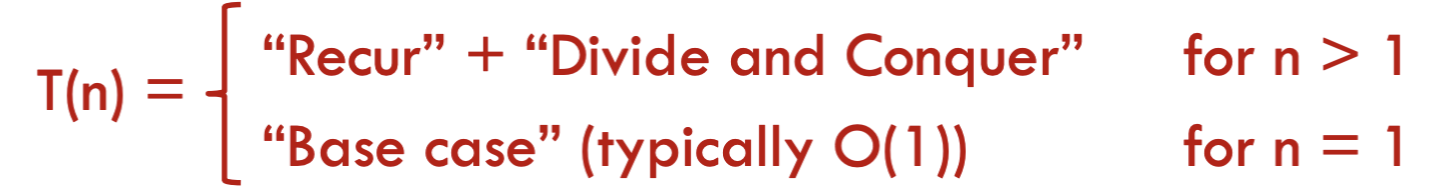
\includegraphics[width=0.8\textwidth]{image28.png} 

% Section 3  ----------------------------------------------------------------------------------------
\section{Unrolling}
\begin{center}
  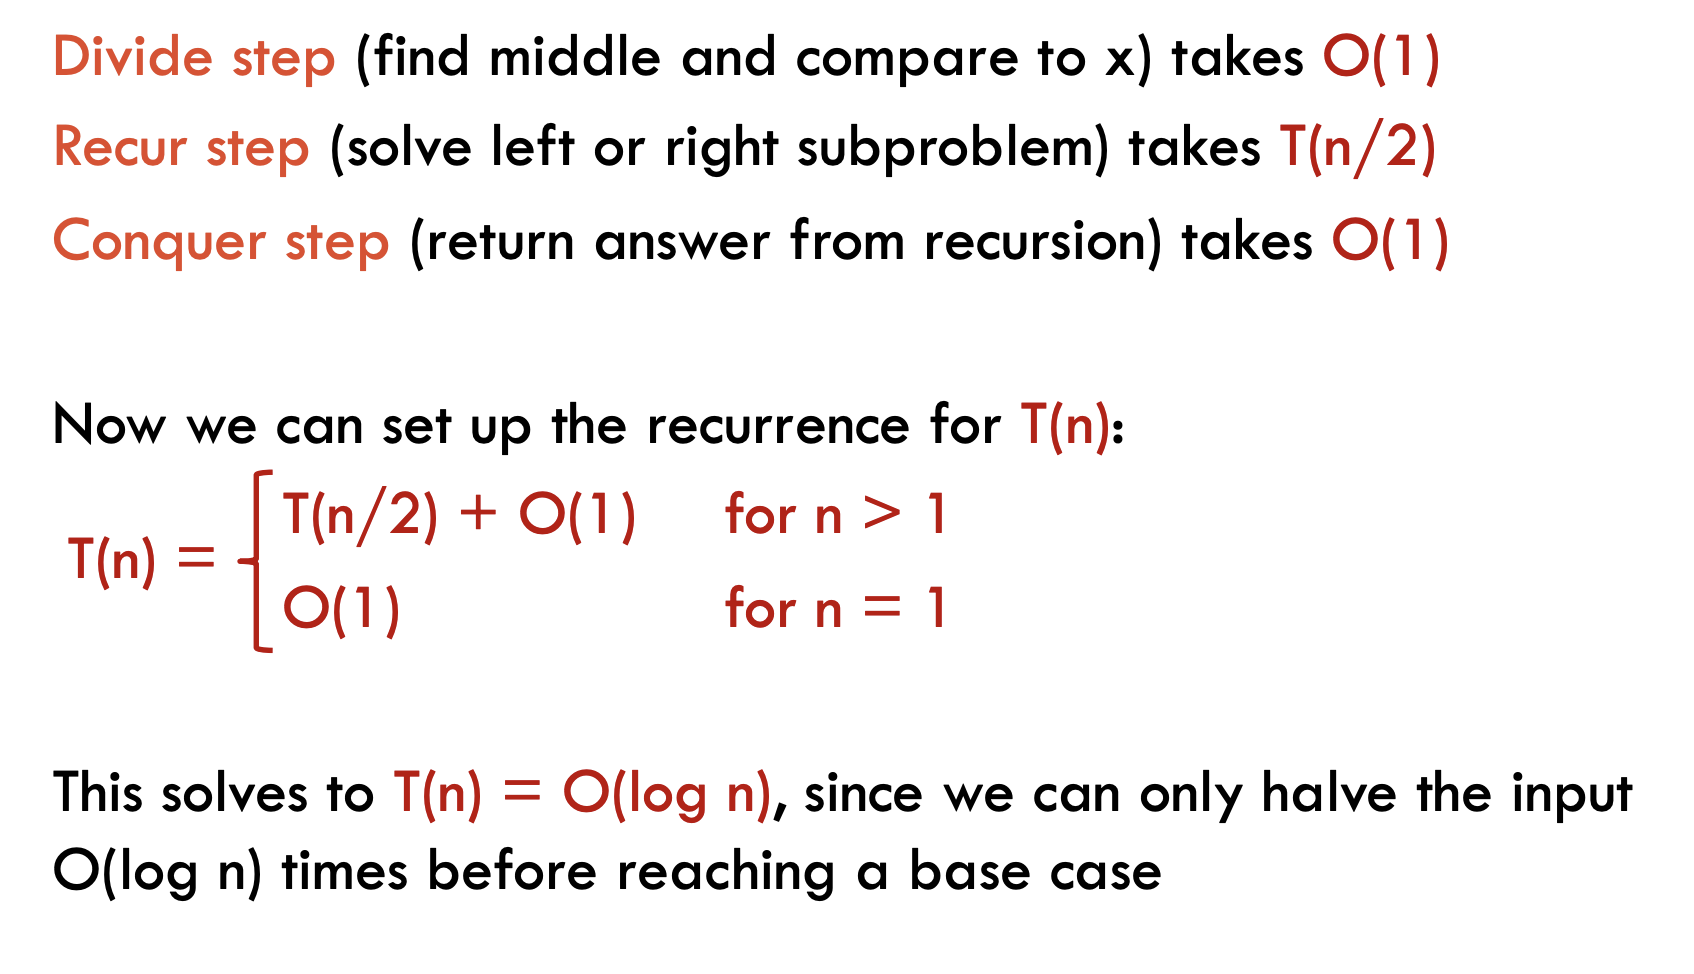
\includegraphics[width=0.7\textwidth]{image29.png} 
\end{center}

\begin{center}
  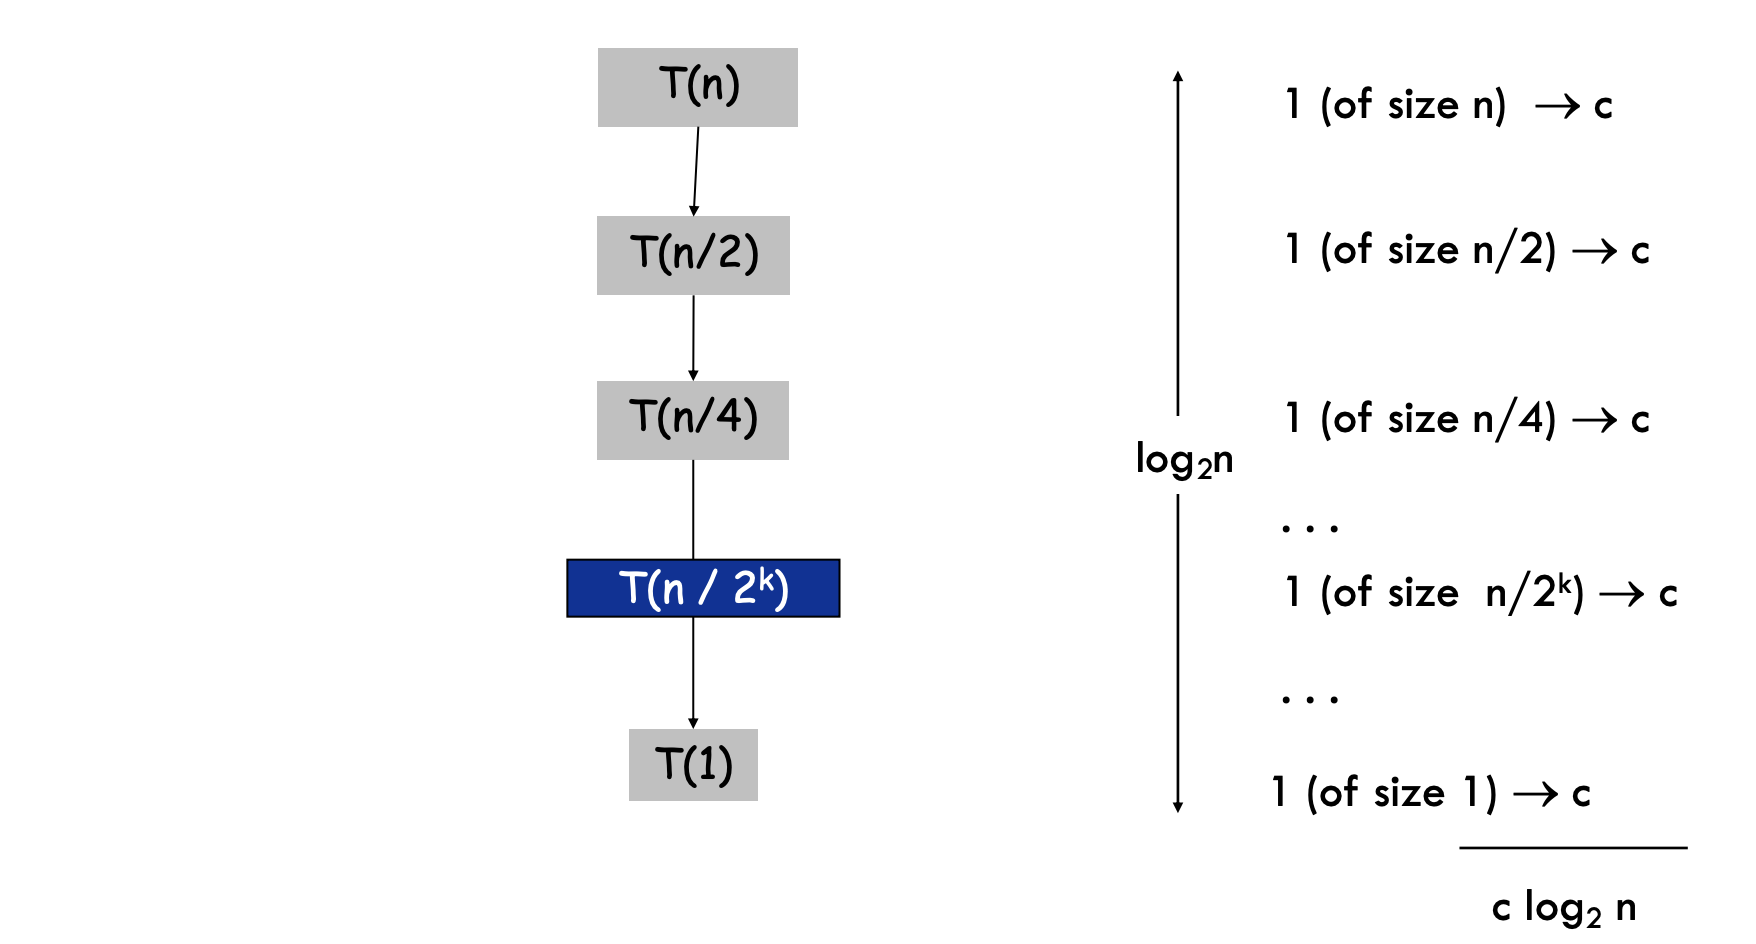
\includegraphics[width=0.85\textwidth]{image30.png} 

  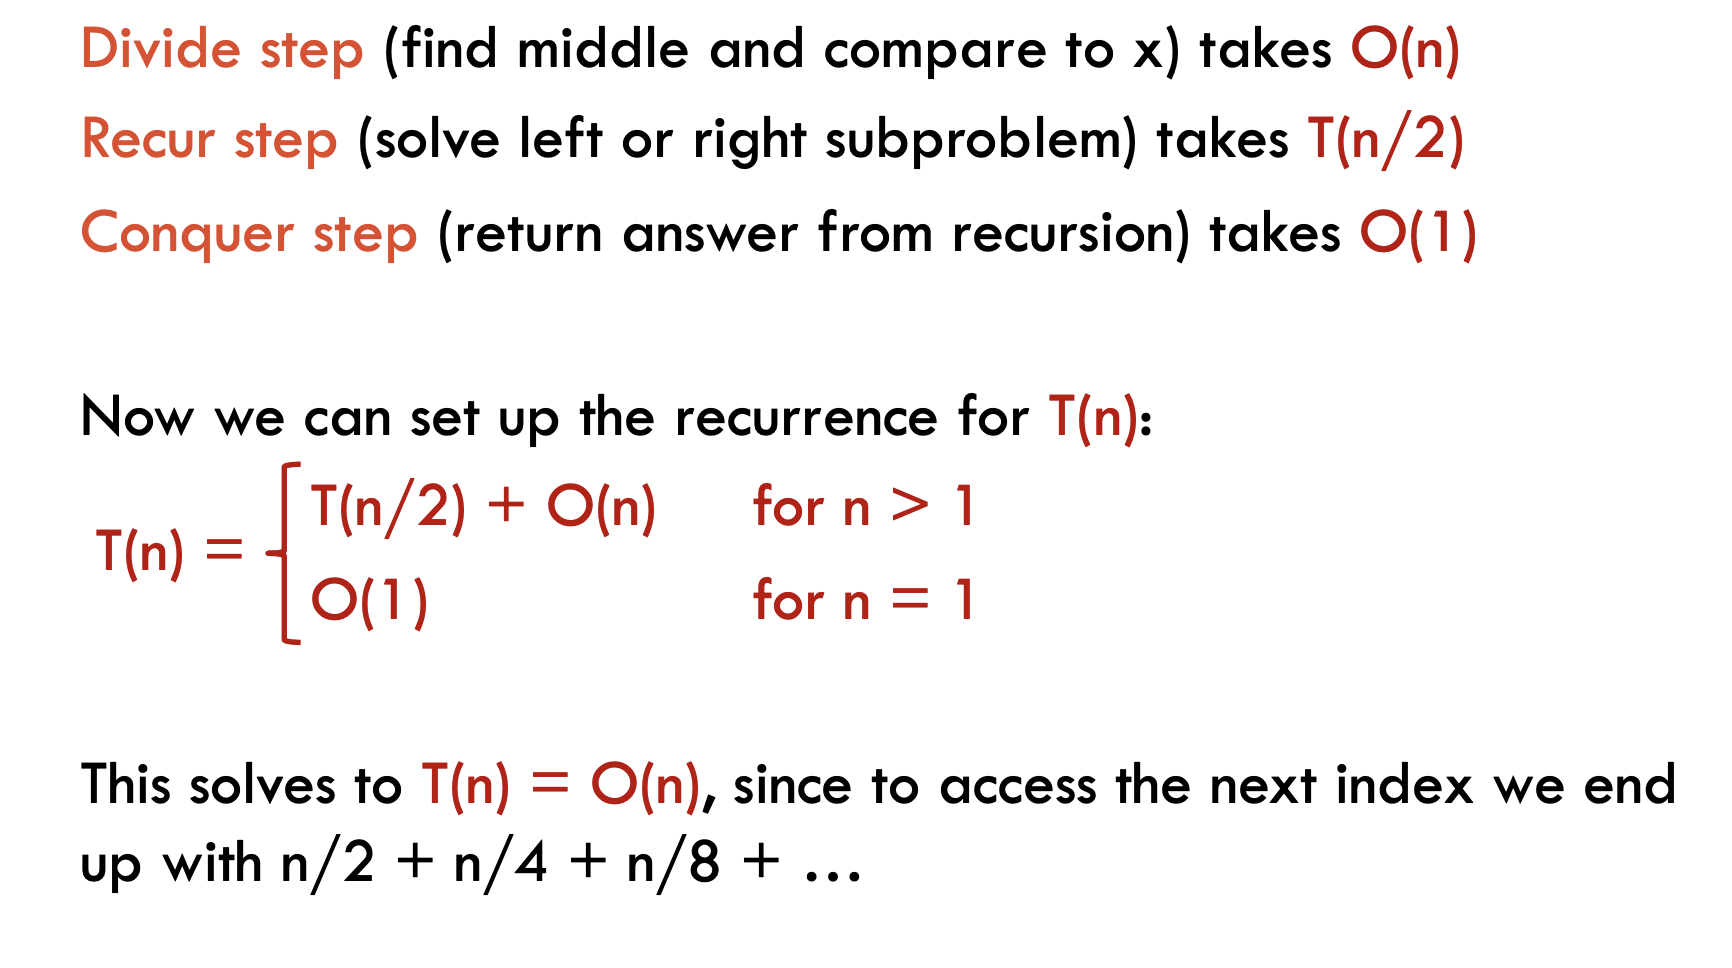
\includegraphics[width=0.85\textwidth]{image31.png} 

  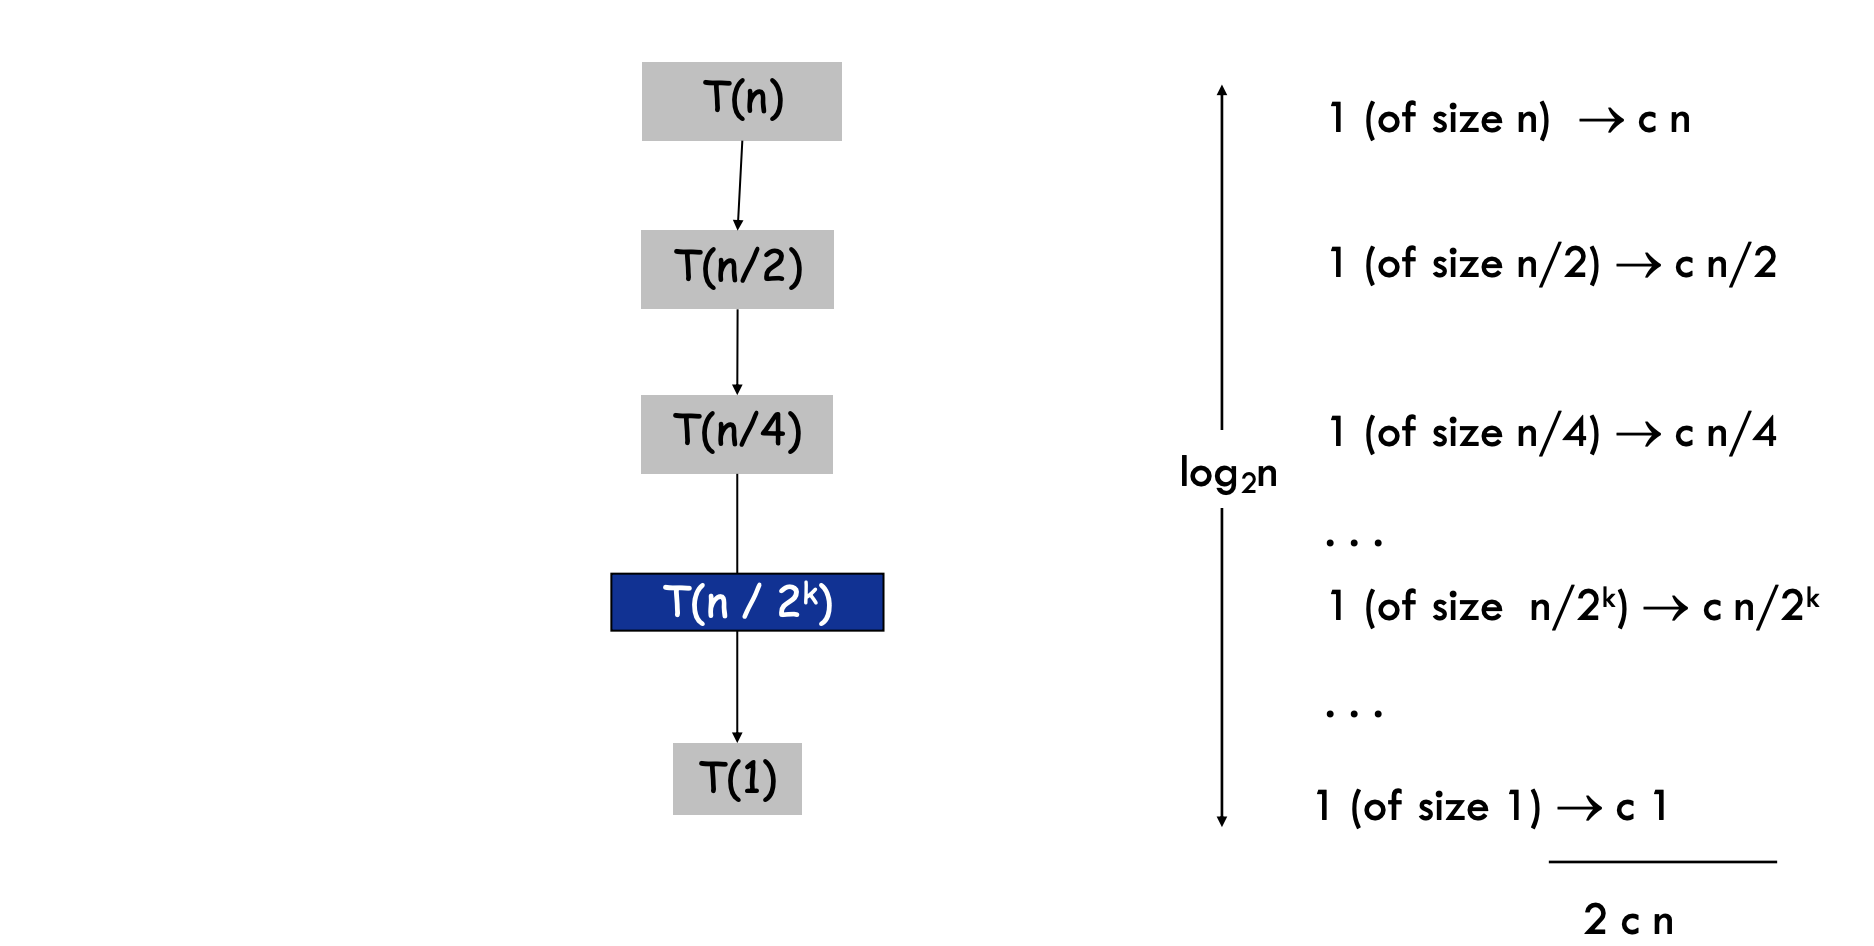
\includegraphics[width=0.85\textwidth]{image32.png} 
\end{center}

% Section 4  ----------------------------------------------------------------------------------------
\section{Merge-Sort}
Divide the array into two halves. Recurrsively sort each half. Conquer two sorted halves to make a single 
sorted array.

\begin{pseudo}
  \I \DEF{merge\_sort}{s}
  \I \1 \IF{|S| < 2} \comment{base case}
  \I \2 \return{s}
  \I \1 \ELSE
  \I \2 mid \assign $\lfloor |S| \div 2 \rfloor$ \comment{divide}
  \I \2 left \assign S[:mid]
  \I \2 right \assign S[mid:]
  \I \2 sorted\_left \assign merge\_sort(left) \comment{recursion}
  \I \2 sorted\_right \assign merge\_sort(right)
  \I \2 \return{merge(sorted\_left, sorted\_right)} \comment{conquer}
\end{pseudo}

\begin{pseudo}
  \I \DEF{merge}{L, R}
  \I \2 result \assign array of length (|L| + |R|)
  \I \2 l, r \assign $0$, $0$
  \I \2 \while{l + r < |result|}
  \I \3 index \assign l + r
  \I \3 \IF{r >= |R| \textbf{or} (l < |L| \textbf{and} L[l] < R[r])}
  \I \4 result[index] \assign L[l]
  \I \4 l \assign l + 1
  \I \3 \ELSE
  \I \4 result[index] \assign R[r]
  \I \4 r \assign r + 1
  \I \2 \return{result}
\end{pseudo}

\subsection{Merge Correctness}
\textbf{Induction hypothesis:} After the i-th iteration, our result contains the i smallest elements in sorted 
order.

\vspace{10pt}
\textbf{Base case:} After $0$ iterations, our result is empty, so it contains the 0 smallest elements in sorted 
order.

\vspace{10pt}
\textbf{Induction:} Assume IH after iteration k. RTP to prove it after iteration k+1.
Since both halves are sorted and we add the smallest element not
already in result, result now contains the k+1 smallest elements.
Sorted order follows from the fact that both halves are sorted, thus
adding the smallest element implies sorted order of result.

\subsection{Merge-Sort Correctnes}
\textbf{Induction hypothesis:} Merge-Sort correctly sorts an array of size i

\vspace{10pt}
\textbf{Base case:} If our array has size 0 or 1, it’s already sorted.

\vspace{10pt}
\textbf{Induction:} Assume IH for all arrays up to size k. RTP it for array of size k+1.
Splitting the array in half gives us two array of size at most k, so by IH
those are sorted correctly. We proved that given two sorted arrays, Merge returns a correctly
sorted array containing the elements of both arrays. Hence, by running Merge on the two sorted 
halves, we sort the original array.

\subsection{Merge sort complexity analysis}
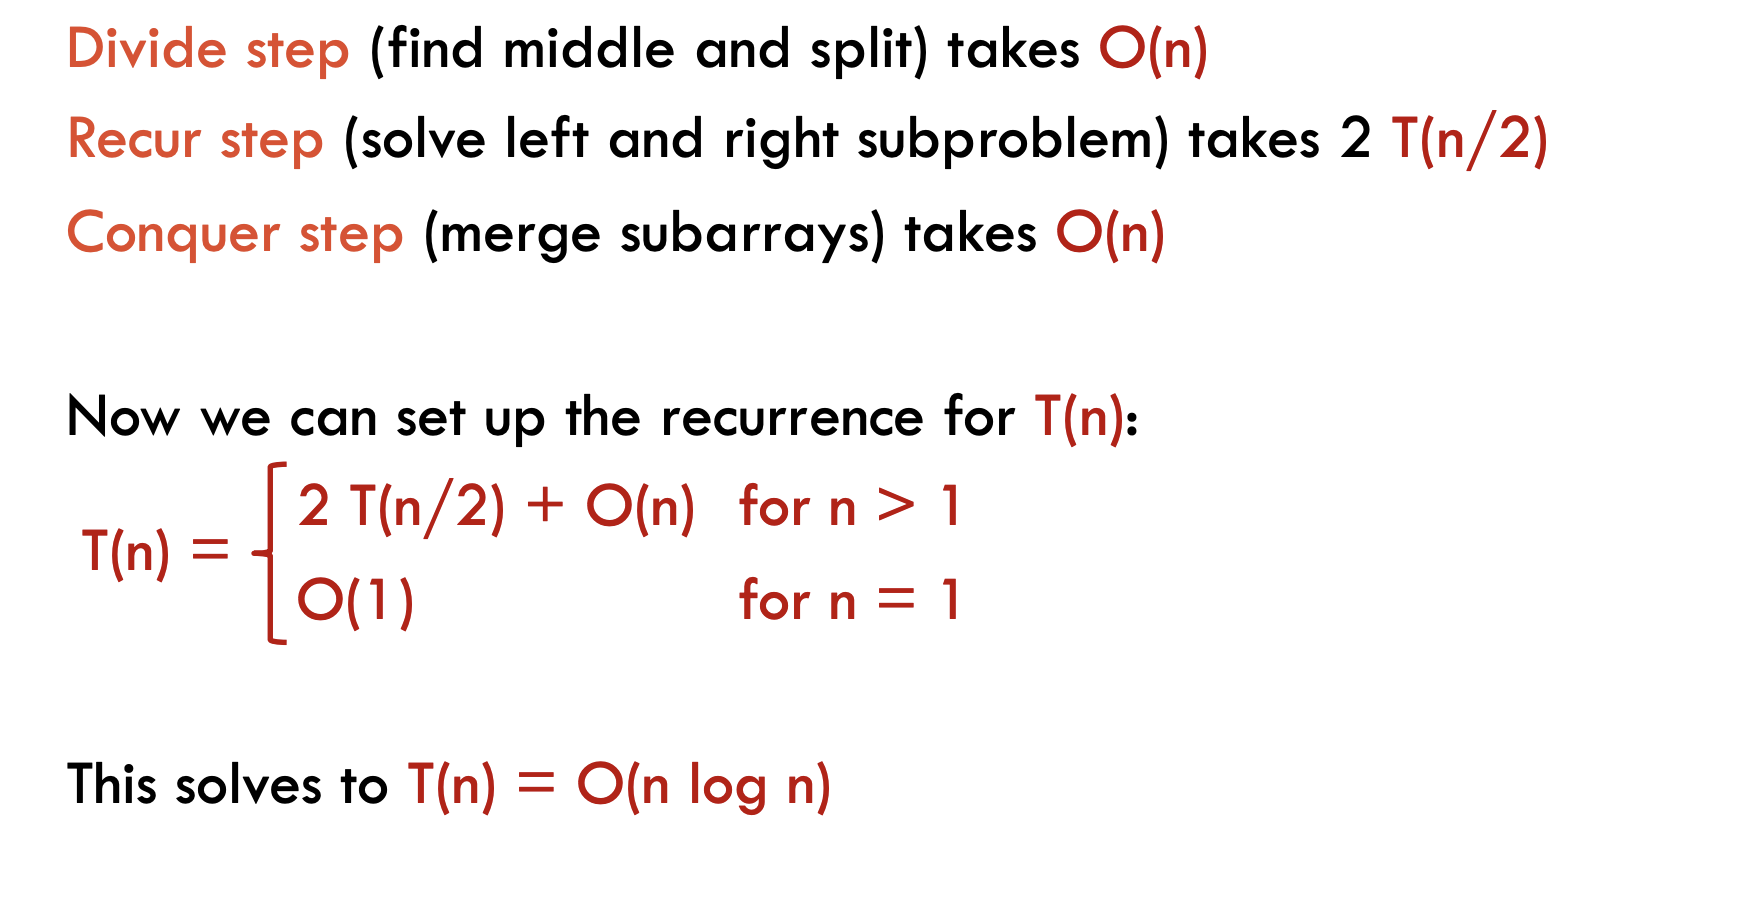
\includegraphics[width=0.85\textwidth]{image33.png} 

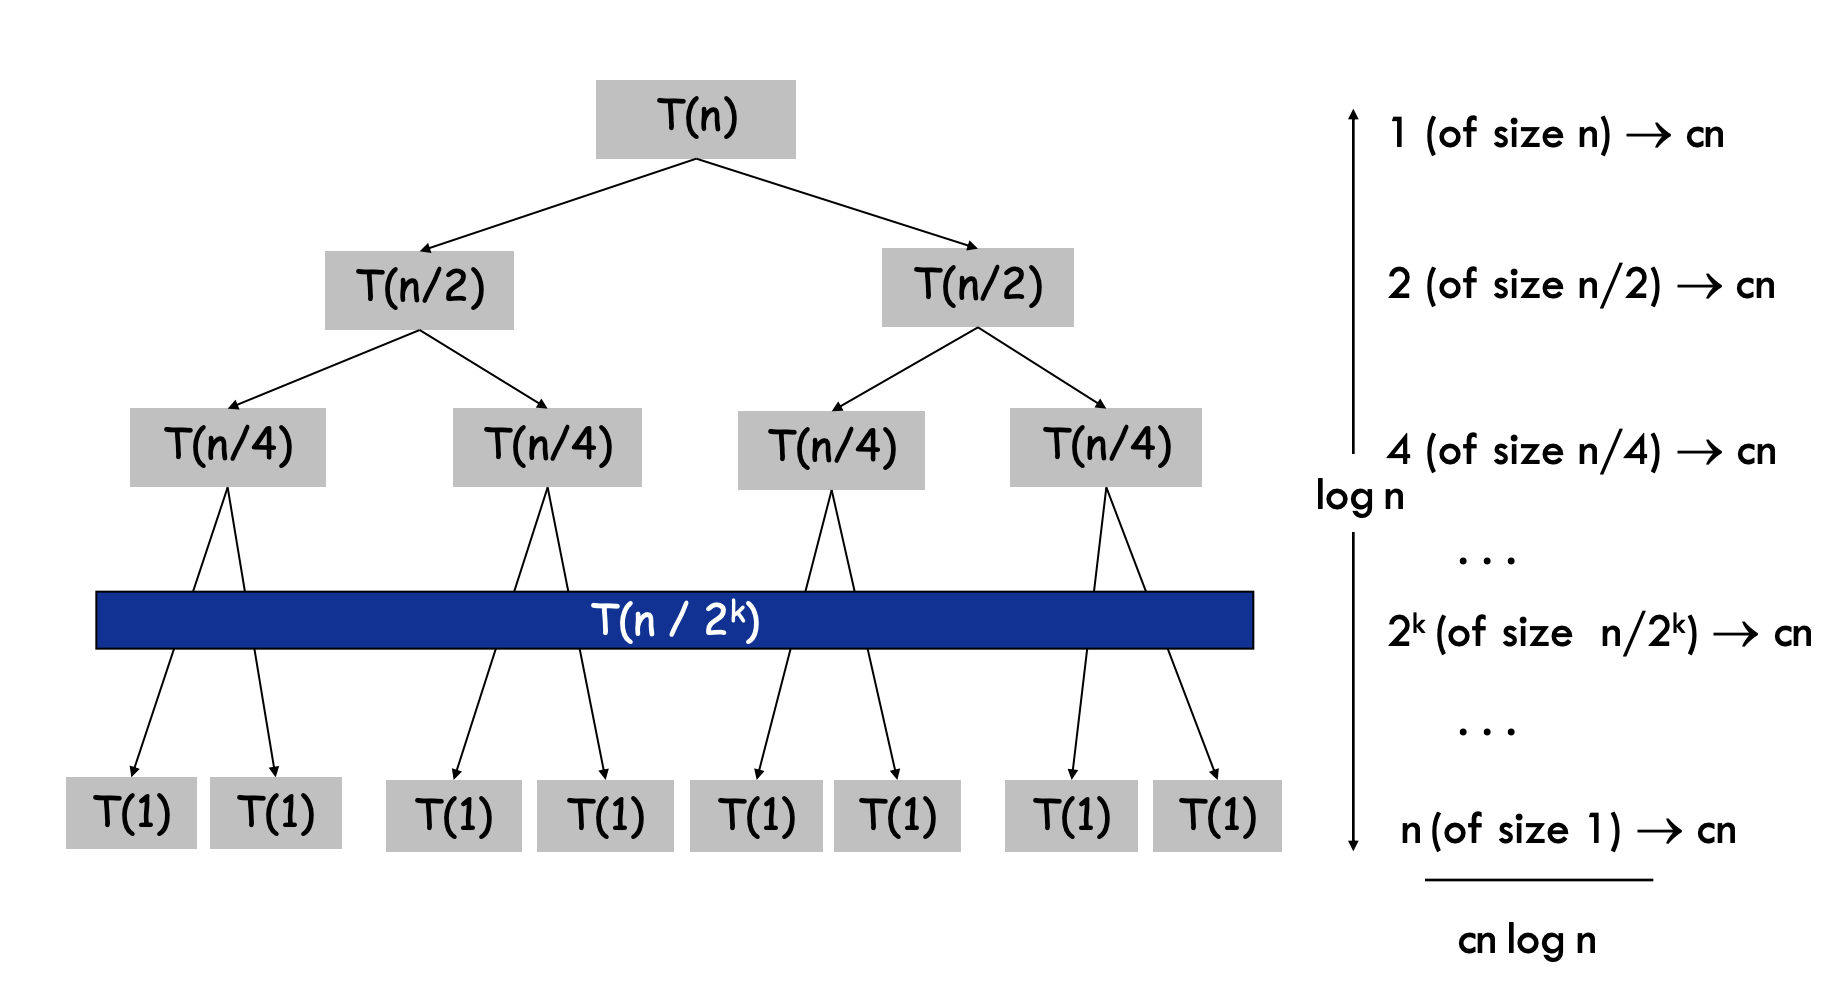
\includegraphics[width=0.85\textwidth]{image34.png} 

% Section 5  ----------------------------------------------------------------------------------------
\section{Quick sort}
\begin{enumerate}
  \item \textbf{Divide:} Choose a random element from the list as the pivot. Partition the elements into 
  3 lists: (i) less than, (ii) equal to and (iii) greater than the pivot.
  \item \textbf{Recursively sort:} Recursively sort the less than and greater than lists.
  \item \textbf{Conquer:} Concatenate the 3 sorted lists.
\end{enumerate}

\subsection{Quick sort complexity analysis}
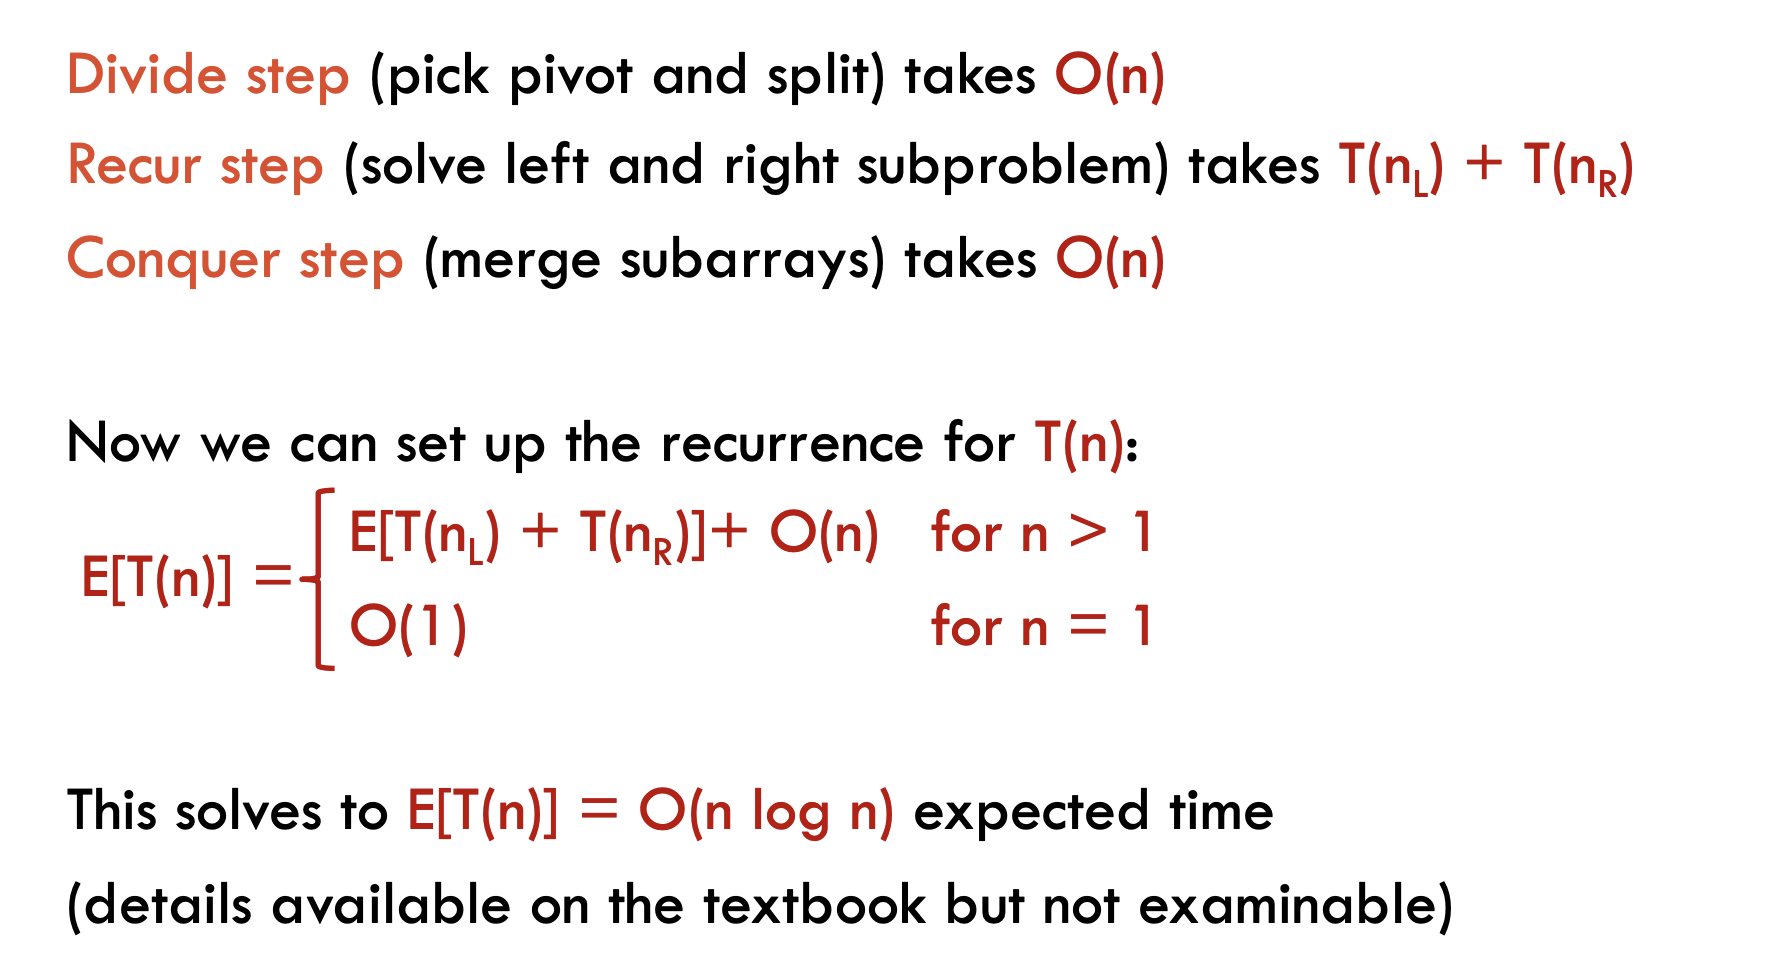
\includegraphics[width=\textwidth]{image35.png} 

% Section 6  ----------------------------------------------------------------------------------------
\section{Other notes on divide and conquer}

\textbf{Important:}
Simply using Merge-Sort in your algorithm doesn’t make your algorithm a divide and conquer algorithm. 
For example, A greedy algorithm could use merge sort for its sorting step.

\subsection{Comparison sorting lower bound}
\textbf{Fact:} Comparison-based sorting algorithms take $\Omega(n \log n)$ time.

\vspace{10pt}
\textbf{Proof:}
The decision tree associated with a comparison-based sorting algorithm is binary and has $n!$ external nodes. Thus, the height is $\log n!$, which is $\Omega(n \log n)$.


\subsection{Some recurrence formulas with solutions}
\begin{tabular}{|l|l|}
  \hline
  \rowcolor{myBlue}
  \color{white}{\textbf{Recurrence}} \hspace{165pt} & \color{white}{\textbf{Solution}} \hspace{165pt} \\
  \hline
  T(n) = 2 T(n/2) + O(n) & T(n) = O(n log n) \\
  \hline
  T(n) = 2 T(n/2) + O(log n) & T(n) = O(n) \\
  \hline
  T(n) = 2 T(n/2) + O(1) & T(n) = O(n) \\
  \hline
  T(n) = T(n/2) + O(n) & T(n) = O(n) \\
  \hline
  T(n) = T(n/2) + O(1) & T(n) = O(log n) \\
  \hline
  T(n) = T(n-1) + O(n) & T(n) = O($n^2$) \\
  \hline
  T(n) = T(n-1) + O(1) & T(n) = O(n) \\
  \hline
\end{tabular}

% Section 7  ----------------------------------------------------------------------------------------
\section{Maxima-Set (Pareto frontier)}
\textbf{Definition:} A point is maximum in a set if all other points in the set have either a smaller x- or smaller 
y-coordinate. 

\textbf{Problem:} Given a set S of n distinct points in the plane (2D), find
the set of all maximum points.

\begin{enumerate}
  \item \textbf{Preprocessing:} Sort the points by increasing x coordinate and store them in an array. 
  Note: we only do this once. Break ties in x by sorting by increasing y coordinate.
  \item \textbf{Divide:} Split the sorted array into two halves.
  \item \textbf{Recur:} Recursively find the maximum points in each half.
  \item \textbf{Conquer:} Merge the two sets of maximum points.
\end{enumerate}
\begin{center}
  \includegraphics*[width=0.8\textwidth]{image36.png}
\end{center}

\subsection{Maxima-Set: Analysis}
\begin{center}
  \includegraphics*[width=\textwidth]{image37.png}
\end{center}

\subsection{Maxima-Set: Correctness}
\begin{center}
  \includegraphics*[width=\textwidth]{image38.png}
\end{center}

% Section 8  ----------------------------------------------------------------------------------------
\section{Integer multiplication}
\begin{pseudo}
  \I \DEF{multiply}{x, y}
  \I \1 \IF{x = $0$ \textbf{or} y = $0$} \return{$0$} \comment{base case}
  \I \1 \IF{x = $1$} \return{y}
  \I \1 \IF{y = $1$} \return{x}
  \I \1 let $x_1$ and $x_0$ be such that x = $x_1$ $2^{n / 2}$ + $x_0$
  \I \1 let $y_1$ and $y_0$ be such that y = $y_1$ $2^{n / 2}$ + $y_0$
  \I \1 \return{multiply($x_1$, $y_1$) $2^n$ + (multiply($x_1$, $y_0$) + multiply($x_0$, $y_1$)) $2^{n / 2}$
  \NL \1 \, + multiply($x_0$, $y_0$)}
\end{pseudo}
\includegraphics*[width=0.9\textwidth]{image39.png}

\includegraphics*[width=0.9\textwidth]{image40.png}

\subsection{Attempt 2}
\includegraphics*[width=0.9\textwidth]{image41.png}

\begin{pseudo}
  \I \DEF{multiply}{x, y}
  \I \1 \IF{x = $0$ \textbf{or} y = $0$} \return{$0$} \comment{base case}
  \I \1 \IF{x = $1$} \return{y}
  \I \1 \IF{y = $1$} \return{x}
  \I \1 first\_term \assign multiply($x_1$, $y_1$)
  \I \1 last\_term \assign multiply($x_0$, $y_0$)
  \I \1 other\_term \assign multiply($x_1$ + $x_0$,$y_1$ + $y_0$)
  \I \1 \return{first\_term $2^n$ + (other\_term - first\_term - last\_term) $2^{n / 2}$ + last\_term}
\end{pseudo}

\includegraphics*[width=\textwidth]{image42.png}

% Section 9  ----------------------------------------------------------------------------------------
\section{Math concepts to remember}

\textbf{Base exchange rule:}
\[
\log_a x = \frac{\log_b x}{\log_b a}
\]

\textbf{Product rule:}
\[
\log_a (xy) = \log_a x + \log_a y
\]

\textbf{Power rule:}
\[
\log_a x^b = b \log_a x
\]

\textbf{Let $r$ be +real and $k$ a +integer}
\[
1 + r + r^2 + \ldots + r^k = \frac{{r^{k+1} - 1}}{{r - 1}}
\]

\textbf{Consequently, if $r > 1$}
\[
1 + r + r^2 + \ldots + r^k < \frac{{r^{k+1}}}{{r - 1}}
\]

\textbf{and if $r < 1$}
\[
1 + r + r^2 + \ldots + r^k < \frac{1}{{1 - r}}
\]

% Section 10  ----------------------------------------------------------------------------------------
\section{Quick selection}
\begin{center}
  \includegraphics*[width=0.8\textwidth]{image43.png}
\end{center}
\begin{center}
  \includegraphics*[width=\textwidth]{image44.png}
\end{center}
\end{document}